\chapter{Geografía y teoría económica}

\section{Introdución}

\textbf{La agrupación de actividades económicas se puede encontrar en varios niveles de agregación:} la variación considerable en el tamaño económico de las ciudades o regiones a nivel nacional, o la distribución desigual de la riqueza y la producción a nivel mundial.\\
Surge la pregunta de por qué la ubicación parece ser tan importante para las actividades económicas. Para responder a esta pregunta, necesitamos un marco analítico en el que la geografía juegue un papel de una forma u otra.\\
Las ciudades y regiones varían en tamaño y relevancia. Este es un tema primordial para la economía regional y urbana y también para la geografía económica propiamente dicha, que tradicionalmente se ocupa del análisis teórico de las interdependencias entre ciudades y regiones dentro de un país.\\\\
\begin{center}
    ¿qué tiene que decir cada teoría sobre el papel de la geografía?
\end{center}

\section{La geografía en la economía regional y urbana}
\textbf{La economía regional analiza la dispersión espacial y la coherencia de la actividad económica}
\textbf{La economía regional (también conocida como ciencia regional) se basa en la teoría económica neoclásica y es, en efecto, la sucesora formalizada de la tradición alemana de la economía de ubicación. La geografía económica, por otro lado, es más ecléctica y orientada empíricamente.} Se inspira en teorías económicas heterodoxas y, cada vez más, en áreas externas a la economía, como la sociología, las ciencias políticas y la teoría de la regulación. Comenzamos con una descripción general de un campo de estudio más joven, a saber, \textbf{la economía urbana, que estudia la estructura espacial de las áreas urbanas.} Al igual que la economía regional, la economía urbana se basa en gran medida en las herramientas del análisis neoclásico, de modo que la división entre economía regional y urbana no siempre es clara. 

\subsection{La economía urbana}

\textbf{La distribución desigual de la actividad económica dentro de cada país es el punto de partida de la economía urbana.} El análisis moderno de la aglomeración de empresas y personas en ciudades o áreas metropolitanas se basa en gran medida en \textbf{la economía de la aglomeración, un término que se refiere a la disminución de los costos promedio a medida que se produce una mayor producción dentro de un área geográfica específica. En otras palabras, se basa en rendimientos crecientes a escala.} Antes de entrar en la relevancia de las economías de escala para las ciudades y otras formas de aglomeración, primero analizamos un modelo en el que no hay rendimientos crecientes a escala. Este modelo, el modelo de ciudad monocéntrica. Se justifica una breve discusión, aunque solo sea para poder notar las diferencias con el enfoque de la economía geográfica y dejar claro que, al final, el análisis de las ciudades seguirá siendo bastante limitado mientras no haya rendimientos crecientes a escala.

\subsubsection{El modelo de la ciudad monocéntrica}
El modelo de ciudad monocéntrica asume la existencia de un plano sin rasgos distintivos, perfectamente plano y homogéneo en todos los aspectos. En medio de este plano hay una sola ciudad. Fuera de la ciudad, los agricultores cultivan cultivos que deben vender en la ciudad. Hay costos de transporte positivos asociados con llevar los productos agrícolas a la ciudad, que difieren para los diversos cultivos, al igual que los precios de estos cultivos. Se  analiza cómo los granjeros se ubican a través del plano. \textbf{Cada agricultor quiere estar lo más cerca posible de la ciudad para minimizar sus costos de transporte.} Este incentivo de estar cerca de la ciudad da como resultado mayores rentas de la tierra cerca de la ciudad que en el borde del plano. Por lo tanto, \textbf{cada agricultor se enfrenta a una compensación entre las rentas de la tierra y los costos de transporte.}\\
\textbf{Se demostró que la competencia por las ubicaciones garantiza que la asignación de tierras equilibrada resultante entre los agricultores sea eficiente.} Para cada tipo de cultivo existe una curva de oferta-renta que indica, dependiendo de la distancia a la ciudad, cuánto están dispuestos a pagar los agricultores por la tierra. Dado que las curvas de oferta-renta difieren por cultivo, como resultado de los diferentes precios de esos cultivos en la ciudad y los diferentes costos de transporte, los agricultores de un tipo particular de cultivo pueden superar a sus competidores (es decir, están dispuestos a pagar más) \textbf{para cualquier distancia dada a la ciudad. A medida que nos alejamos del centro de la ciudad,  vemos que, primero, los productores de flores superan la oferta de los otros dos grupos de agricultores, luego que entre los puntos A y B los productores de vegetales están dispuestos a pagar las rentas más altas y que a la derecha del punto B (y por lo tanto el más alejado del centro de la ciudad) los productores de granos pagarán la renta más alta.} Esto da como resultado un patrón de círculos concéntricos de uso de la tierra alrededor de la ciudad, cada anillo consta de granjas que cultivan el mismo cultivo; en secuencia: flores, vegetales y granos.\\
La economía urbana probablemente comenzó como una disciplina separada con William Alonso (1964), quien tomó el modelo de von Thunen y, esencialmente, reemplazó la ciudad por un centro comercial central y los agricultores por viajeros. Los viajeros viajan de ida y vuelta a su trabajo en el centro de negocios, y cada viajero obtiene utilidad de su espacio para vivir, pero también enfrenta costos de transporte. Nuevamente, las rentas de la tierra son las más altas cerca de la ciudad y disminuyen con la distancia. Por lo tanto, se puede aplicar el enfoque de oferta y renta, y la competencia por la tierra entre los viajeros implica una asignación eficiente de la tierra. La eficiencia de la asignación de tierras en el modelo monocéntrico depende del supuesto de que no hay externalidades de ubicación. Combinado con el trabajo de Richard Muth (1969) y Mills (1967), el modelo de Alonso (1964) es sigue siendo la columna vertebral de la economía urbana moderna.\\
Una serie de hechos estilizados sobre la estructura espacial urbana están de acuerdo con el modelo monocéntrico. Primero, la densidad de población disminuye con la distancia de los centros comerciales centrales. En segundo lugar, casi todas las ciudades importantes del mundo occidental se descentralizaron en el siglo XX (a medida que la gente comenzó a ubicarse más lejos del centro de la ciudad), lo que puede estar relacionado con una caída en los costos de transporte. \textbf{El modelo monocéntrico también tiene algunas limitaciones serias. Mencionamos solo dos. Primero, el modelo no tiene en cuenta ninguna interacción entre ciudades; no puede ocuparse de los sistemas urbanos. Segundo, el modelo toma la existencia y ubicación de la ciudad como dadas y se enfoca en la ubicación de agricultores/viajeros fuera de la ciudad.} La pregunta de por qué hay una ciudad para empezar queda sin respuesta. Para hacer frente a estas limitaciones, los economistas urbanos han reconocido durante mucho tiempo que una teoría de las ciudades no puede prescindir de la introducción y el fundamento teórico de algún tipo de rendimientos crecientes a escala. Estos pueden ocurrir a nivel de empresa o a un nivel más agregado (el nivel de la industria o el nivel nacional). 

\paragraph{Economías de escala externas e internas}
\textbf{El término economías de escala o rendimientos crecientes a escala se refiere a una situación en la que un aumento en el nivel de producción implica una disminución en los costos promedio por unidad de producción para la empresa. Se traduce en una curva de costo promedio con pendiente negativa. Para identificar el origen de la caída de los costes medios, se distingue entre economías de escala internas y externas. Con las economías de escala internas, la disminución de los costes medios se produce por un aumento del nivel de producción de la propia empresa.} Cuanto más produce la empresa, mejor puede beneficiarse de las economías de escala y mayor es su ventaja de costos sobre las empresas más pequeñas. \textbf{La estructura de mercado que subyace a las economías de escala internas, típicamente utilizada en la literatura de economía geográfica, debe ser necesariamente de competencia imperfecta, ya que las economías de escala internas implican poder de mercado.} Con \textbf{las economías de escala externas, la disminución de los costes medios se produce a través de un aumento de la producción a nivel de la industria en su conjunto, lo que hace que los costes medios por unidad sean una función de la producción de toda la industria. Scitovsky distingue aquí entre economías externas puras y pecuniarias.}\\
\textbf{Con economías externas puras (o tecnológicas), un aumento en la producción de toda la industria altera la relación tecnológica entre insumos y producción para cada empresa individual. Por lo tanto, tiene un impacto en la función de producción de la empresa.} Un ejemplo de uso frecuente (que se remonta a Alfred Marshall; se refiere a los derrames de información. Un aumento en la producción de la industria aumenta el acervo de conocimiento a través de los efectos indirectos positivos de información para cada empresa, lo que lleva a un aumento en la producción a nivel de empresa. \textbf{En la economía urbana, pero también en la nueva teoría del crecimiento  y la nueva teoría del comercio , se supone que existen economías externas puras. La estructura del mercado puede entonces ser perfectamente competitiva ya que el tamaño de la empresa individual no importa.}\\
\textbf{Las economías externas pecuniarias son transmitidas por el mercado a través de efectos de precio para la empresa individual, lo que puede alterar su decisión de producción.} Dos ejemplos, de nuevo basados en Marshall, son la existencia de un gran mercado local de insumos especializados y la puesta en común del mercado laboral. Una gran industria puede respaldar un mercado de insumos intermedios especializados y un grupo de trabajadores calificados específicos de la industria, lo que beneficia a la empresa individual. \textbf{A diferencia de las economías externas puras, estos efectos indirectos no afectan la relación tecnológica entre insumos y productos (la función de producción). Las externalidades pecuniarias existen en la literatura de economía geográfica a través de un efecto de gusto por la variedad en un gran mercado local. La utilidad de cada consumidor depende positivamente del número de variedades que puede comprar de un bien manufacturado. Los efectos de precio cruciales para las externalidades pecuniarias solo pueden ocurrir con competencia imperfecta. Esto es consistente con el requisito de competencia imperfecta para las economías de escala internas, también utilizado en la literatura de economía geográfica.}\\
Algunas observaciones finales están en orden. Primero, los derrames o externalidades son cruciales para las economías externas. El concepto de derrames a veces se utiliza solo para economías externas puras, refiriéndose a las economías externas pecuniarias como un caso de interdependencia del mercado. Nos ceñimos al uso de derrames o externalidades cuando nos referimos a economías de escala externas en general. De manera similar, el término rendimientos crecientes a veces se usa solo para economías de escala internas. También usamos la frase rendimientos crecientes cuando hablamos de economías externas. Del contexto quedará claro si nos referimos al nivel de la empresa o de la industria.\\

\begin{center}
    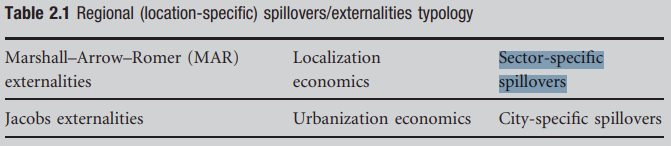
\includegraphics[scale=0.5]{imagen/imagen1.png}
\end{center}

\textbf{En segundo lugar, las economías externas pueden aplicarse a un nivel de agregación superior al de la empresa. Este suele ser el nivel de la industria, pero en la teoría moderna del comercio y la teoría moderna del crecimiento también puede ser la economía en su conjunto. Tercero, las economías externas en los modelos son estáticas, mientras que la literatura también considera economías externas dinámicas.} En ese caso, los costos promedio por unidad de producción son una función negativa de la producción acumulada de la industria. Nuevamente, si esto es relevante, quedará claro si nos referimos a economías externas estáticas o dinámicas. \textbf{Cuarto, las economías externas discutidas anteriormente son positivas,  también pueden ser negativos, es decir, un aumento en la producción de una empresa conduce a un aumento en los costos por unidad para otras empresas.}\\
Finalmente, una observación sobre la terminología un tanto confusa con respecto a las externalidades económicas regionales o efectos indirectos. Es habitual distinguir entre las externalidades Marshall-Arrow-Romer (MAR) y las externalidades de Jacobs. En ambos casos, el énfasis está en los efectos indirectos regionales (específicos de la ubicación), es decir, las empresas deben estar ubicadas lo suficientemente cerca unas de otras para beneficiarse de estas externalidades. Las externalidades SAM se centran en los efectos indirectos específicos del sector y también se conocen como economía de localización. Las externalidades de Jacobs se centran en los efectos indirectos específicos de la ciudad que cruzan los límites entre sectores individuales. Estos también se conocen como economía de la urbanización. 


\subsubsection{Economía urbana y rendimientos crecientes}
\textbf{A diferencia del modelo de ciudad monocéntrica, se incluyen rendimientos crecientes a escala. El punto de partida es bastante diferente del modelo monocéntrico. No hay costes de transporte y el interior de una ciudad ya no forma parte del análisis.} En cierto sentido, es un análisis de las ciudades en las que el espacio, es decir, el espacio fuera de las ciudades, no tiene ningún papel que desempeñar. \textbf{La justificación de este descuido geográfico del espacio no urbano es que, en los países industrializados modernos, una gran parte de la actividad económica general y de la población se encuentra en áreas urbanas, de modo que la relevancia de lo urbano frente a lo no urbano Se supone que las transacciones son limitadas.} En cambio, \textbf{el análisis se centra en las fuerzas que determinan el tamaño de las ciudades y las interacciones entre ellas. Las fuerzas de aglomeración en el modelo de Henderson son economías de escala externas positivas que son específicas de la industria. Esto último significa que hay derrames positivos cuando una empresa de una industria en particular se ubica en una ciudad donde se encuentran otras empresas de la misma industria.} Usando una categorización bien conocida que se remonta a los trabajos de Marshall, estos pueden deberse a:
\begin{enumerate}[\bfseries (i)]
    \item El intercambio de información, 
    \item la existencia de una gran cantidad de mano de obra, o
    \item la existencia de especialistas proveedores.
\end{enumerate}
Por lo tanto, las economías externas pueden, en principio, involucrar economías externas puras (como en el enfoque original de Henderson) o economías externas pecuniarias. \\
Las fuerzas de expansión son economías de escala externas negativas dentro de la ciudad, como la congestión, que es una función del tamaño total de la ciudad. Una ciudad grande implica costos de transporte y rentas de la tierra relativamente altos. Las deseconomías de escala no dependen del tipo de producción que se lleva a cabo en la ciudad, por lo que dependen únicamente del tamaño total de una ciudad. Junto con las economías externas específicas de la industria, esto tiene dos implicaciones importantes. En primer lugar, puede racionalizar los sistemas de ciudades (diferentes tamaños de ciudades que satisfacen las necesidades de diferentes industrias). Basado en el supuesto de que los efectos secundarios positivos de la ubicación son específicos de la industria, cada industria tiene su propio tamaño óptimo. Ciudades de diferentes tamaños comercian entre sí. En comparación con el marco de von Thunen o Alonso, la economía urbana moderna es mucho menos ad-hoc porque puede brindar una base teórica para los rendimientos crecientes que impulsan la existencia de las ciudades, y produce conocimientos sobre los sistemas urbanos. 

\subsubsection{¿Qué tipo de economías de escala externas?}
Existe un amplio respaldo empírico para la idea de que los efectos indirectos específicos de la industria son importantes para las ciudades. \textbf{Estas economías externas específicas de la industria se conocen como economías de localización, a diferencia de las economías de urbanización. Las últimas son economías externas que se aplican a empresas de todos los sectores y captan la noción de efectos indirectos positivos para una empresa como resultado de la actividad económica total en una ciudad. Ambos tipos de economías externas a menudo se relacionan con la ubicación de las ciudades en un sentido estático, pero también se aplican en un contexto dinámico (¿cómo se desarrollan las ciudades con el tiempo?).} Con respecto al crecimiento de las ciudades en los Estados Unidos, no encuentran apoyo para la hipótesis de que las ciudades especializadas en ciertas industrias crecen más rápidamente en promedio. En cambio, concluyen que \textbf{si las economías externas son importantes, probablemente sea más importante tener una variedad de industrias diversificadas en una ciudad.} Si este último es el caso, surge la pregunta de por qué tantas ciudades están especializadas en industrias particulares. Se sugieren que tanto las economías de localización como las de urbanización son relevantes (aunque al final favorecen las economías de urbanización), mientras que otros argumentan que en un contexto dinámico las economías de localización son más relevantes.\\
Desde un punto de vista teórico, cabe destacar que el enfoque de los sistemas urbanos de Henderson no da por sentada la existencia de la ciudad, como hacía el modelo monocéntrico. También proporciona una teoría de las interacciones entre ciudades. \textbf{El problema con el enfoque es que el espacio fuera de las ciudades (deliberadamente) no forma parte del análisis. Esto es problemático si uno quiere poder decir dónde están ubicadas las ciudades en relación con otras y la parte no urbana de la geografía:} La literatura sobre sistemas de ciudades ha enfatizado el espacio urbano pero ha descuidado el espacio nacional. Como veremos, \textbf{la ubicación de la actividad manufacturera y la relación entre estas ubicaciones y el resto del espacio es un tema clave en la economía geográfica. Para analizar esta relación, los costos de transporte deben ser parte del análisis, ya que son cruciales para determinar el equilibrio entre las fuerzas de aglomeración y expansión.}\\
En sus estudios de las teorías de la aglomeración, que incluye la economía urbana, \textbf{se analizan tres enfoques básicos: rendimientos crecientes, externalidades y competencia espacial.} Su uso de rendimientos crecientes y externalidades corresponde a nuestra definición de economías externas puras y economías externas pecuniarias, respectivamente. Ambos tipos de economías externas son importantes. Esto deja la competencia espacial, lo que significa que \textbf{la competencia entre empresas es casi automáticamente de naturaleza oligopólica cuando se toma en consideración el espacio.} La competencia está restringida por la distancia; Por lo general, se piensa que una empresa compite solo con sus empresas vecinas. \textbf{La competencia espacial está, por tanto, intrínsecamente ligada al comportamiento estratégico de las empresas. La razón es simplemente que en la economía geográfica y en particular en la versión de competencia monopolística, que caracteriza la estructura del mercado en nuestro modelo central de economía geográfica, el comportamiento estratégico no es tenido en cuenta.} Las empresas toman el comportamiento (fijación de precios) de las demás como dado. Además de los tres enfoques mencionados dan dos razones adicionales para la aglomeración (urbana): la existencia de un espacio no homogéneo y economías de escala internas en un proceso de producción. Con el primero se puede racionalizar la aglomeración sin ninguna forma de rendimientos crecientes a escala (piense en las diferencias en la geografía física real que da lugar, por ejemplo, a un puerto natural y la aglomeración correspondiente).

\subsection{Economía regional}
\textbf{La economía regional analiza la organización espacial de los sistemas económicos (y no solo de las ciudades) y de alguna manera también debe dar cuenta de la distribución desigual en el espacio.} Todas las contribuciones alemanas toman en consideración el espacio nacional o de toda la economía para analizar dónde se ubican las actividades económicas. Esta es una pregunta relevante ya que el movimiento de bienes y personas no es gratuito y la producción suele estar sujeta a alguna forma de rendimientos crecientes. Sin embargo, los padres fundadores de la economía regional se centran en diferentes aspectos de la ubicación de la actividad económica. Como vimos, von Thunen, por ejemplo, enfatizó las decisiones de ubicación tomadas por los agricultores, mientras que Weber analizó la ubicación óptima y el tamaño de la planta para las empresas manufactureras. Esta subsección se centra en las ideas presentadas (y probadas) por primera vez por Christaller y Losch, quienes trataron no solo de explicar la ubicación de las ciudades sino también de diferenciarlas por las diversas funciones que desempeñan y de tratar las relaciones entre las ciudades y el medio ambiente. No ciudades. Este enfoque se conoce como la teoría del lugar central, que muestra que diferentes puntos o ubicaciones en el panorama económico tienen diferentes niveles de centralidad y que los bienes y servicios se proporcionan de manera eficiente sobre una base jerárquica.\\

\subsubsection{Teoría del lugar central}
\textbf{Dada una distribución uniforme de consumidores idénticos en un plano homogéneo, la teoría del lugar central sostiene que las ubicaciones difieren en centralidad y que esta centralidad determina el tipo de bienes que proporciona la ubicación.} La provisión de estos bienes está determinada por rendimientos internos crecientes a escala, mientras que la ubicación es relevante porque los consumidores incurren en costos de transporte. Para minimizar estos costos, los consumidores quieren tener acceso a proveedores de bienes cercanos. Para algunos tipos de bienes, como el pan, esto es más fácil que para otros, como los televisores, porque los rendimientos crecientes a escala son relativamente limitados. Por lo tanto, la economía puede sustentar muchos lugares relativamente pequeños (pueblos) donde los panaderos están activos para suministrar pan. Por el contrario, solo puede haber relativamente pocos lugares (ciudades pequeñas, los lugares centrales) donde las empresas de electrónica vendan televisores, que la gente compra con menos frecuencia. Para minimizar los costos de transporte, ambos tipos de ubicaciones se distribuyen de manera bastante uniforme en el espacio. Además, obtenemos una jerarquía de lugares donde la ciudad realiza todas las funciones (vende pan y televisores), mientras que el pueblo realiza solo algunas funciones (vende solo pan). Donde el lugar central equidistante está rodeado por seis equidistantes ciudades más pequeñas, que juntas forman un hexágono. Cada ciudad pequeña, a su vez, está rodeada por seis aldeas equidistantes.\\
El hecho de que se ocupe explícitamente de la ubicación de la actividad económica es una ventaja importante de la teoría del lugar central. El principal problema con el enfoque es que la lógica económica detrás de las decisiones de los consumidores y las empresas sigue sin estar clara. ¿Qué tipo de comportamiento de los agentes individuales conduce a un resultado de lugar central? Los rendimientos crecientes a nivel de empresa requieren alguna forma de competencia imperfecta, un análisis que falta. En consecuencia, la teoría del lugar central, especialmente la versión gráfica que todavía se encuentra en la mayoría de los libros de texto de introducción a la geografía económica, es más una historia descriptiva que un modelo causal.\\
Por supuesto, los científicos regionales y los geógrafos económicos también han sido conscientes de las limitaciones de esta versión de la teoría del lugar central, que durante los últimos treinta años ha recibido menos interés, particularmente dentro de la geografía económica. Para una base teórica, los geógrafos económicos han comenzado a buscar en otra parte. Y también explicamos por qué los geógrafos económicos modernos son bastante críticos con el trabajo realizado por los economistas geográficos (y viceversa). Sin embargo, siguiendo a Walter Isard (1956, 1960), los científicos regionales han tratado de construir sobre las ideas básicas de la teoría del lugar central para dar una base económica teórica (a menudo altamente formalizada) a esta teoría. Estos modelos son en su mayoría de naturaleza de equilibrio parcial, explicando algunos aspectos del sistema de lugar central mientras ignoran otros. \textbf{Por lo general, un modelo en esta tradición no trata con empresas o consumidores individuales, sino que formaliza esencialmente el patrón geométrico de un sistema de lugar central}. El resultado del lugar central es, por lo tanto, meramente racionalizado y no explicado por el comportamiento subyacente de los consumidores y productores, ni por sus decisiones e interacciones (de mercado). Por ejemplo, la curva de demanda que enfrenta una empresa en un lugar particular no se deriva de los primeros principios, sino que simplemente se supone. \textbf{La economía geográfica intenta llenar este vacío en la literatura dando una base microeconómica a la jerarquía de los lugares centrales.} 

\paragraph{Teoría del lugar central en un pólder holandés}
Entre 1937 y 1942, se recuperó del mar un área de 48 000 hectáreas (120 000 acres) y se convirtió en un pólder en el centro de los Países Bajos. El nuevo pólder, llamado Noord-Oost Polder (Polder del noreste), fue y sigue siendo utilizado principalmente para la agricultura. Las autoridades holandesas también planificaron el establecimiento de una serie de (pequeños) pueblos y aldeas en este pólder, y su planificación estuvo explícitamente influenciada por el trabajo de Christaller y Losch en lugares centrales. El pólder cumplió claramente con algunos de los supuestos de la teoría del lugar central: la tierra es extremadamente plana y casi perfectamente homogénea en todos los demás aspectos. Los colonos iniciales en el pólder (los granjeros) también estaban distribuidos uniformemente por todo el pólder, y no era demasiado descabellado suponer que estos granjeros tenían preferencias idénticas. El desembolso de las nuevas ubicaciones en el pólder, se parecía mucho al desembolso del lugar central. Había un lugar central (la ciudad de Emmeloord), que quedó rodeada durante un período de diez años por varios lugares más pequeños (casi) equidistantes. Estas ubicaciones más pequeñas se diseñaron explícitamente para suministrar solo bienes de orden inferior, mientras que Emmeloord se diseñó para suministrar  bienes de orden superior (para el desembolso de los distintos lugares en el pólder). Con base en esta idea central de la teoría del lugar central, las autoridades hicieron proyecciones sobre el tamaño de cada lugar. Estas proyecciones se eliminaron de la realidad después de sesenta años. El lugar central se había vuelto mucho más grande de lo previsto, algunas ubicaciones son casi correctas y algunas ubicaciones se han vuelto más pequeñas de lo esperado. 

\subsubsection{Potencial de mercado}
\textbf{Las observaciones anteriores sobre el fundamento de la teoría del lugar central se aplican de manera más general. Hay más ejemplos de teorías que, como la teoría del lugar central, intentan enfrentarse a una regularidad espacial pero que carecen de un fundamento económico-teórico convincente.} A diferencia de la teoría económica (neoclásica), existe una tendencia a dar simplemente una representación, utilizando, por ejemplo, ecuaciones simples, de la regularidad sin conexión con un modelo del comportamiento individual subyacente de los agentes económicos. Otros ejemplos de modelos utilizados para describir o imitan regularidades espaciales empíricas particulares son (i) las ecuaciones subyacentes a la distribución de rango-tamaño , (ii) el modelo de gravedad del comercio , y (iii) \textbf{el análisis del potencial de mercado . Este último, debido a Chauncy Harris (1954), es ampliamente utilizado en economía regional. Para el caso de los Estados Unidos, y utilizando el valor de las ventas minoristas por condado de los EE. UU., Harris encuentra que el potencial de mercado de cualquier ubicación se puede describir mediante}

\begin{equation}
    MP_i = \sum_{j=1}^n \dfrac{M_j}{D_{ij}}
\end{equation}

Donde $MP_i$ es el mercado potencial de la ubicación $i$, $M_j$ es la demanda de la ubicación $j$ por los bienes de la ubicación $i$, y $D_{ij}$ es la distancia entre las ubicaciones $i$ y $j$.\\
Por lo tanto, la ecuación del potencial de mercado proporciona una indicación de la proximidad general de una ubicación en relación con la demanda total. Harris (1954), y muchos economistas regionales desde entonces, \textbf{han descubierto que el potencial de mercado (y por lo tanto la demanda) suele ser alto en aquellas áreas donde también se encuentra realmente la producción. Esto respalda la noción de agrupamiento de la actividad económica e indica que las decisiones de aglomeración y ubicación en las que se basa no son solo un problema del lado de la oferta, sino que la demanda también juega su papel. De hecho, la idea de que la producción tiene lugar donde la demanda es alta también puede revertirse. La demanda es alta donde se ubica la producción como resultado del poder adquisitivo de los trabajadores que hacen posible la producción en ese lugar.} Aunque convincente desde un punto de vista empírico, \textbf{el análisis del potencial de mercado carece de una base teórica (y por lo tanto también carece de contenido: ¿qué representa MPi?). Esto no es muy sorprendente, porque la teoría del crecimiento y el comercio económico tienen grandes dificultades para explicar cualquier fenómeno en el que la geografía juega un papel.} En particular, la variable de distancia $D_{ij}$ es difícil de reconciliar con la teoría económica. \textbf{Sin embargo, las ideas detrás del análisis del potencial de mercado juegan un papel destacado en la economía geográfica, el modelo central de la economía geográfica puede interpretarse como un intento de proporcionar una base teórica para la ecuación (2.1). El trabajo empírico en economía geográfica también utiliza el enfoque del mercado potencial}.\\
Ambos ejemplos (la teoría del lugar central y el enfoque del potencial de mercado) ilustran algunos puntos que se aplican de manera más general. Los enfoques teóricos, como la teoría del lugar central, y los enfoques de inspiración más empírica, como el análisis del potencial de mercado, tratan aspectos importantes del espacio espacial. Organización de la actividad económica. Sin embargo, el marco de análisis en general no cumple con los estándares de la teoría económica dominante, que requiere que las conclusiones se basen en las acciones e interacciones de los agentes económicos individuales en el mercado. Esto requiere el análisis del comportamiento individual del consumidor y del productor, la estructura del mercado y los equilibrios resultantes. Tal fundamento microeconómico de la geografía no existe (o simplemente no se consideró útil para empezar) en algunos rincones de la economía regional.  

\subsection{¿Es nueva la economía geográfica? La mirada desde la economía urbana y regional}
\textbf{La economía geográfica puede verse como una nueva geografía económica en la medida en que combina percepciones espaciales bien establecidas de la economía regional y urbana con el marco de equilibrio general de la teoría económica dominante.} Intenta no sólo poner más teoría económica en geografía pero, sobre todo, más geografía en la economía convencional, mientras se utiliza el conjunto de herramientas de la economía convencional. Si este intento produce nuevos conocimientos sobre las relaciones entre la geografía y la economía o solo fundamenta el trabajo existente (y, para algunos geógrafos económicos, obsoleto) en un marco analítico diferente, es una cuestión diferente. Antes de volver a la corriente principal de la teoría económica del comercio y el crecimiento y su análisis (o falta de él) de la geografía en el resto de este capítulo, es útil hacer las siguientes dos observaciones sobre el legado de la economía urbana y regional para la economía geográfica y su intento de fundamentar el análisis de la distribución de la actividad económica a través del espacio en un marco de equilibrio general.\\
\textbf{La primera observación es que el marco estándar de equilibrio general no funcionará si queremos que importen la geografía o el espacio. La existencia de costos positivos de transporte o comercio dará como resultado un equilibrio en el que no habrá transporte ni comercio de bienes.}\\
Como veremos en la siguiente sección, la opción de la no homogeneidad del espacio es la ruta tradicionalmente tomada por la teoría del comercio internacional. Las teorías sobre economía urbana y regional discutidas en la presente sección toman la segunda ruta. Con von Thunen, la fricción o la no divisibilidad requerida para llegar a un resultado de equilibrio significativo en un mundo de costos de transporte positivos es la suposición de que la producción debe venderse en el mercado central. En la economía urbana y regional moderna, suele ser la introducción de alguna forma de rendimientos crecientes la que desempeña este papel. Fujita y Thisse se refieren a \textbf{las fuerzas económicas rendimientos crecientes: costos de transporte como la compensación fundamental para una economía espacial. Como veremos en los capítulos 3 y 4, esto también es válido para la economía geográfica.} Con rendimientos crecientes pero sin costos de transporte, a las empresas les puede resultar rentable producir en una sola planta, pero no les importa la ubicación de esta planta. Como argumentamos anteriormente, en ausencia de rendimientos crecientes (o espacio no homogéneo) pero con costos de transporte, terminaremos en una situación de capitalismo de traspatio.\\
\textbf{La segunda observación relacionada es que, debido a que resultó difícil combinar los costos de transporte, los rendimientos crecientes a escala y la competencia imperfecta en un marco de equilibrio general, tomó bastante tiempo desde Koopmans (1957), pasando por Starrett (1978) ) para llegar al primer modelo de economía geográfica, de Krugman (1991a).} Dicho esto, también está claro que muchos de los ingredientes de la economía geográfica no son nuevos y ya eran bien conocidos en 1991, cuando Krugman publicó su modelo en The Journal of Political Economy. En su estudio de la teoría de la aglomeración, Ottaviano y Thisse (2004) plantean la pregunta ¿Dónde estábamos en 1990?, que es anterior a Krugman (1991a). Observan que, con una excepción crucial, todos los elementos importantes ya estaban flotando en la teoría de ubicación existente. Cada ubicación preferirá la autarquía para ahorrar en costos de transporte y, si cada actividad económica es perfectamente (y sin costo) divisible en el espacio, la autarquía o el capitalismo de traspatio con consumidores/trabajadores autoproductivos es el único resultado factible. Esto va, por supuesto, en contra de los hechos más básicos, a saber, que efectivamente observamos comercio entre ubicaciones y la ausencia de capitalismo de traspatio. Por lo tanto, Duranton (2008) concluye: Si uno toma los costos de transporte como un hecho inevitable de la vida, debe asumir alguna no homogeneidad del espacio o alguna no convexidad de los conjuntos de producción. más específicamente, el legado de la teoría de la ubicación se puede resumir en los siguientes cinco puntos (Ottaviano y Thisse, 2004: 2576; énfasis en el original):

\begin{enumerate}[\bfseries (i)]
    \item El espacio económico es el resultado de una compensación entre varias formas de rendimientos crecientes y diferentes tipos de costos de movilidad;
    \item la competencia de precios, los altos costos de transporte y el uso del suelo fomentan la dispersión de la producción y el consumo; por lo tanto;
    \item es probable que las empresas se concentren en grandes áreas metropolitanas cuando venden productos diferenciados y los costos de transporte son bajos; 
    \item las ciudades ofrecen una amplia gama de bienes finales y mercados laborales especializados que las hacen atractivas para los consumidores/trabajadores; y
    \item las aglomeraciones son el resultado de procesos acumulativos que involucran tanto a la oferta como a la demanda.
\end{enumerate}

\textbf{En consecuencia, la economía espacial debe entenderse como el resultado de la interacción entre las fuerzas de aglomeración y dispersión,} una idea propuesta por geógrafos y científicos regionales hace mucho tiempo, dentro de un marco de equilibrio general que explica explícitamente las fallas del mercado.\\
\textbf{Estos cinco puntos también están en el corazón de la economía geográfica, lo que plantea la pregunta de cuál es la diferencia clave entre la economía geográfica al estilo de Krugman (1991a) y las teorías de ubicación existentes de los enfoques urbano y regional.  De hecho, la respuesta es que lo que faltaba era un marco de equilibrio general con competencia imperfecta que conectara estos diversos conocimientos y permitiera un estudio detallado de sus interacciones. La principal contribución de la economía geográfica es, por lo tanto, combinar los elementos existentes en un solo marco analítico}. 

\paragraph{El teorema de la imposibilidad espacial}
\textbf{El teorema de la imposibilidad espacial establece que en una economía con un número finito de ubicaciones y un número finito de consumidores y empresas, en la que el espacio es homogéneo y el transporte es costoso, no existe un equilibrio perfectamente competitivo en el que tenga lugar el transporte real.} Esto es intuitivamente fácil de entender, ya que en tal economía los costos de transporte siempre pueden evitarse porque la producción y el consumo pueden tener lugar a un nivel arbitrariamente pequeño, sin costos adicionales (una situación denominada capitalismo de traspatio en la literatura). En tal mundo hipotético de perfecta divisibilidad, sería imposible explicar por qué ocurre la agrupación o aglomeración de actividades (como observamos en la realidad). \textbf{Sólo si hay indivisibilidades, o costos adicionales involucrados si la producción se divide, la ubicación de las actividades económicas se vuelve importante;} Starrett (1978: 27) afirma: “Mientras haya algunas indivisibilidades en el sistema (de modo que las operaciones individuales deban ocupar espacio), entonces un conjunto suficientemente complicado de actividades interrelacionadas generará costos de transporte. Este principio se conoce como el teorema de imposibilidad espacial de Starrett; \\
Es interesante notar que Tjalling Koopmans señaló hace medio siglo que solo podemos comenzar a comprender la importancia de la ubicación o la geografía para la economía si reconocemos el hecho de que las actividades económicas no son infinitamente divisibles; o, en palabras de Koopmans (1957: 154; énfasis en el original), Sin reconocer las indivisibilidades en la persona humana, en las residencias, plantas, equipos y en el transporte, los patrones de ubicación, hasta los de la aldea más pequeña, no se pueden entender.\\
\textbf{Cada ubicación preferirá la autarquía para ahorrar en costos de transporte y, si cada actividad económica es perfectamente (y sin costo) divisible en el espacio, la autarquía o el capitalismo de patio trasero con consumidores/trabajadores autoproductivos es el único resultado factible.} Esto va, por supuesto, en contra de los hechos más básicos, a saber, que efectivamente observamos comercio entre ubicaciones y la ausencia de capitalismo de traspatio. Por lo tanto, Duranton (2008) concluye: \textbf{Si uno toma los costos de transporte como un hecho inevitable de la vida, debe asumir alguna no homogeneidad del espacio o alguna no convexidad de los conjuntos de producción}.

\section{Teoría del comercio internacional}
En esta sección se analiza el papel de la geografía en la teoría del comercio internacional. \textbf{El modelo central de la economía geográfica tiene sus raíces firmemente en la teoría del comercio internacional. En muchos sentidos es una extensión de la llamada nueva teoría del comercio, específicamente de Krugman (1979, 1980)}. Estos dos artículos, junto con Krugman (1991a) el modelo básico de economía geográfica– le valieron el Premio Nobel de economía en 2008.

\subsection{Teoría neoclásica del comercio}
\textbf{La etiqueta teoría neoclásica del comercio se refiere a teorías en las que los flujos comerciales entre naciones se basan en la ventaja comparativa, resultante de las diferencias tecnológicas (David Ricardo) o de la abundancia de factores.} En el modelo de abundancia de factores, desarrollado por Eli Heckscher, Ohlin y Paul Samuelson, la ventaja comparativa está determinada, como sugiere el nombre, por las diferencias entre países en la abundancia relativa de las dotaciones de factores. Basta con pensar en el modelo simple de abundancia de factores (dos bienes, dos países y dos factores de producción), que sigue siendo la columna vertebral de cualquier curso de introducción al comercio internacional. Fue ampliamente utilizado, por ejemplo, en el debate sobre los efectos de la globalización para los mercados laborales de la Organización para la Cooperación y el Desarrollo Económicos (OCDE).\\
Suponga que hay dos países (Norte y Sur), dos bienes transables (ropa y maquinaria) y dos factores de producción (mano de obra altamente calificada y mano de obra poco calificada). Suponga que el Norte está relativamente bien dotado de mano de obra altamente calificada y el Sur de mano de obra poco calificada. La producción de ambos conjuntos de bienes requiere ambos insumos, pero la producción de maquinaria es relativamente intensiva en habilidades. Los consumidores del Norte y del Sur tienen preferencias idénticas y consumen ambos bienes. En ausencia de comercio, el Norte, que abunda en mano de obra altamente calificada, puede fabricar maquinaria más fácilmente que el Sur, porque la producción de maquinaria requiere mucha destreza. En la autarquía, esto da como resultado un precio relativamente bajo para la maquinaria en el Norte y la ropa en el Sur. Una vez que el Norte y el Sur comiencen a comerciar, los precios se igualarán, lo que resultará en un precio más alto para la maquinaria en el Norte y un precio más alto para la ropa en el Sur. Como consecuencia, North tendrá una incentivo para especializarse (parcialmente) en la producción de maquinaria. Un razonamiento similar es válido para el sur con respecto a la ropa. Los flujos comerciales resultantes son del tipo interindustrial (comercio de maquinaria para prendas de vestir). Además, \textbf{los precios de los factores se igualarán entre el Norte y el Sur como resultado del comercio.}\\
\textbf{El modelo de abundancia de factores utiliza algunos supuestos específicos adicionales, como competencia perfecta, bienes homogéneos, producción con rendimientos constantes a escala, sin costos de transporte asociados con el comercio de bienes y movilidad de los factores de producción entre industrias, pero no entre países.} Está claro que \textbf{varios de estos supuestos están en desacuerdo con los supuestos clave en la economía regional y urbana, en la que tenemos rendimientos crecientes a escala externos y/o internos, competencia imperfecta, costos de transporte positivos y movilidad de los factores de producción (y las empresas)}. Estos ingredientes son necesarios para dar cuenta de los patrones económicos espaciales. ¿Significa esto que la geografía o la ubicación de la actividad económica no es un problema en la teoría neoclásica del comercio? Bueno, sí y no.\\
Para explicar esta respuesta, es útil distinguir entre la primera y la segunda naturaleza de la economía de la ubicación. \textbf{La ubicación de la actividad económica es relevante en el modelo de abundancia de factores en lo que respecta a la distribución desigual de las dotaciones de factores.} Esta distribución está dada y, por lo tanto, es un determinante de ubicación de primera naturaleza en la terminología de Krugman. \textbf{En nuestro ejemplo, el Norte se especializa en maquinaria y el Sur en ropa como resultado de la distribución geográfica de las dotaciones, lo que se traduce en una distribución desigual de la actividad económica en el espacio global. En este sentido restringido, la geografía importa.}\\
Sin embargo, nos gustaría llegar a esta conclusión de otra manera, a saber, mostrando cómo la relevancia de la ubicación se deriva de las decisiones tomadas por los agentes económicos y sus interacciones y no (solo) de alguna diferencia exógena en la dotación de factores. En otras palabras, \textbf{la ubicación de la producción debería ser una variable endógena, un determinante de ubicación de segunda naturaleza en la terminología de Krugman.} Esta segunda naturaleza está claramente ausente en la teoría de la abundancia de factores. \textbf{La endogenización de las decisiones de ubicación es necesaria para producir la aglomeración de la actividad económica.} Las diferencias en la dotación de factores no pueden implicar un patrón de producción centro-periferia; simplemente conducen a la especialización (en oposición a la aglomeración). El comercio entre países no puede conducir a la desigualdad en el sentido de que la maquinaria y la ropa no pueden aglomerarse en el Norte.\\
El modelo de abundancia de factores conduce a la igualación de los salarios de alta calificación entre el Norte y el Sur (y de manera similar para los salarios de baja calificación). Esta teoría económica se ha utilizado para analizar un fenómeno con un componente geográfico evidente: la globalización y su supuesto impacto en la asignación de la producción y la renta en las economías industrializadas occidentales (Norte). \textbf{La globalización puede definirse como la creciente interdependencia entre países a través del aumento del comercio y/o el aumento de la movilidad de los factores.}\\
Las diferencias relativas en las dotaciones de factores se pueden utilizar para dar una justificación teórica de las diferencias en los patrones de especialización entre países. Otras versiones de la teoría neoclásica del comercio tienen implicaciones similares en lo que se refiere a la relevancia de la geografía. En el modelo ricardiano, la ventaja comparativa, y por lo tanto el patrón comercial, está determinado por las diferencias tecnológicas exógenas entre países. \textbf{Los países se especializan en la producción de aquellos bienes en los que tienen una productividad comparativamente alta, lo que determina la ubicación de la producción.} Nuestra principal objeción al modelo de abundancia de factores también es válida para el modelo ricardiano: en la medida limitada en que la geografía importa, esta relevancia se da de manera exógena. Naturalmente, las diferencias en la dotación de factores o la tecnología pueden ser el resultado de diferencias geográficas. Consideremos, por ejemplo, la tierra como un factor de producción, como en la tradición de von Thunen en economía urbana. La disponibilidad de tierra (fértil) da forma a la ventaja comparativa. De manera similar, la geografía física de un país (acceso al mar, altitud, clima, etc.) también puede ser un determinante subyacente de la ventaja comparativa, que sin duda es válida para el stock de recursos naturales. Se  muestran que tales diferencias geográficas entre países ayudan a explicar las diferencias en el desarrollo económico.\\
El papel limitado de la geografía en la teoría neoclásica del comercio quizás se ilustre mejor con el llamado modelo de factores específicos. Parte de la dotación de factores de un país (mano de obra, por ejemplo) es entonces móvil internacionalmente, mientras que otras partes (tierra y capital, por ejemplo) no lo son. La producción de un determinado bien requiere insumos del factor móvil, así como de un factor inmóvil particular o específico (es decir, normalmente tierra o capital específico del sector). Las diferencias en la dotación de los factores específicos influyen así en el patrón de producción y comercio, con un país que se especializa, ceteris paribus, en la producción del bien que requiere el insumo del factor específico con el que el país está relativamente bien dotado. Existe un vínculo geográfico en la medida en que la distribución de las dotaciones inmóviles está determinada por las condiciones geográficas. Una vez más, tal conexión es indirecta en el mejor de los casos, y el impacto de la geografía se determina fuera del modelo comercial.\\
Para resumir, se afirman correctamente que el espacio no homogéneo, también conocido como espacio no neutral, se ha invocado tradicionalmente para explicar la distribución desigual de la actividad económica en la economía internacional. Estos dan lugar a distintas fuentes de ventaja comparativa, que imposibilitan la expansión de la actividad económica. Por lo tanto, \textbf{la relevancia de la ubicación existe solo por suposición, y no hay interdependencia entre la geografía y la economía. En particular, la ubicación de equilibrio de la actividad económica no es el resultado del comportamiento subyacente de los agentes económicos.} El equilibrio (comercial) suele ser único y totalmente determinado por fuerzas exógenas. Más importante aún, la teoría neoclásica del comercio no permite el establecimiento de un equilibrio centro-periferia, lo que presenta un problema en vista de los muchos ejemplos dados en el capítulo 1. Para permitir la aglomeración de la actividad económica, algunos de los supuestos subyacentes a la teoría neoclásica del comercio han de ser cambiado. Un candidato obvio es la introducción de rendimientos internos crecientes a escala y, por lo tanto, de competencia imperfecta.\\
\textbf{Una observación final sobre la relación entre la geografía y la teoría neoclásica del comercio es que, sin una distribución desigual de los recursos y, por lo tanto, sin una ventaja comparativa, ceteris paribus ya no es una razón fundamental para el comercio, y la geografía deja de ser un problema.} Se puede llegar a una conclusión similar incluso si existen ventajas comparativas. Si estos costos son lo suficientemente altos, la producción de bienes estará perfectamente dispersa en el espacio. La economía consistirá entonces en muchas pequeñas empresas, produciendo para su propio consumo: capitalismo de traspatio nuevamente. Esto se relaciona directamente con la discusión del teorema de imposibilidad espacial, donde concluimos que una salida era introducir un espacio no homogéneo (la ruta tradicionalmente tomada en la teoría del comercio internacional) y otra salida era introducir un espacio no homogéneo. -convexidades en la producción, de las cuales los rendimientos crecientes a escala son el mejor ejemplo. A este respecto, la nueva teoría del comercio que se presenta a continuación tiene más en común con la economía urbana y regional que con la teoría neoclásica del comercio.

\paragraph{Globalización, abundancia de factores y agrupamiento}
Supongamos que el mundo se puede caracterizar con un modelo de abundancia de factores con dos países (Norte y Sur), dos bienes manufactureros (máquinas y prendas de vestir) y un bien no comercializable y no manufacturero. El norte está relativamente bien dotado de mano de obra altamente calificada, el sur con mano de obra poco calificada. Ambos factores de producción son necesarios para la producción de todos los bienes, pero la producción mecánica es relativamente intensiva en habilidades. Por lo tanto, el norte tiene una ventaja comparativa en la producción de máquinas. Ambos países producen bienes transables, hay competencia perfecta, la tecnología es fija y no hay movilidad laboral transfronteriza. Suponga que inicialmente, debido a los costos de transacción muy altos, ambos países no comercian en absoluto. Ahora, los costos de transacción disminuyen y el comercio se abre. La caída en los costos de transacción (que sirve como un indicador de la globalización) puede ser impulsada por políticas (reducción de tarifas y similares) o impulsada por la tecnología (tecnologías mejoradas de transporte y comunicación). ¿Cuáles son los principales efectos del comercio para el Norte? Se especializará en la producción de maquinaria y comenzará a importar prendas de vestir, es decir, el sector de maquinaria se expande y el sector de prendas de vestir se contrae. Esto tiene las siguientes implicaciones para el norte.
\begin{enumerate}[\bfseries (1)]
    \item Habrá un salario de alta calificación y un salario de baja calificación (el teorema de igualación del precio de los factores). Dado que los salarios se determinan en el mercado mundial, los cambios en la oferta nacional de factores ya no tienen ningún impacto en los salarios.
    \item El norte se enfrenta a un aumento de la producción mundial de prendas de vestir, lo que se traduce en una caída del precio relativo de las prendas. Esto perjudicará a la mano de obra poco calificada en el norte, utilizada intensivamente en la producción de prendas de vestir, al reducir su salario real (teorema de Stolper-Samuelson).
    \item La expansión del sector de la maquinaria en el Norte aumenta la demanda relativa de mano de obra altamente calificada, elevando así los salarios de los trabajadores altamente calificados en relación con los salarios de los trabajadores poco calificados en el Norte. Esto induce a las empresas del norte a sustituir la mano de obra altamente calificada y disminuye la intensidad de mano de obra calificada de la producción manufacturera en el norte.
    \item La contracción del sector de la confección en el norte no solo cambia la combinación de la producción manufacturera, sino que también implica una contracción del sector manufacturero en su conjunto, porque parte de la mano de obra liberada del sector de la confección se empleará en el sector no comercializable. Sector servicios. En consecuencia, el sector no manufacturero se expande y el norte se enfrenta a la desindustrialización.
\end{enumerate}
Por lo tanto, se puede recurrir al modelo de abundancia de factores para brindar una base teórica a la idea de que la globalización (aumento de las importaciones por parte del norte de bienes intensivos poco calificados del Sur) puede perjudicar a los trabajadores poco calificados, al reducir sus salarios relativos, y puede conducir a desindustrialización. La principal dimensión geográfica de este análisis de la globalización es la implicación de que el Norte (los países de la OCDE) se especializan en la producción intensiva en mano de obra calificada, mientras que el Sur se especializa en la producción intensiva en mano de obra poco calificada (el sudeste de Asia, América Latina o las economías en transición en Europa del Este).\\
Una pregunta importante para esta versión del debate sobre la globalización es, por supuesto, si existe alguna evidencia empírica que respalde el modelo de abundancia de factores en general para validar las implicaciones 1 a 4 anteriores. El modelo de abundancia de factores ha sido objeto recientemente de una impresionante cantidad de investigación empírica.  Aunque existe cierto desacuerdo, el consenso general parece ser que se necesitan suposiciones adicionales relativamente sólidas para cerrar la brecha entre la teoría neoclásica y los datos. En cualquier caso, las cuatro implicaciones del modelo de abundancia de factores no están fundamentadas de manera convincente por la evidencia empírica. Por lo tanto, es dudoso que el modelo de abundancia de factores (solo) pueda explicar el empeoramiento de la posición de la mano de obra poco calificada en el Norte.

\subsection{Nueva teoría comercial}
Desde finales de la década de 1970 en adelante, la teoría neoclásica del comercio ha sido desafiada por el desarrollo de la nueva teoría del comercio, que ahora es complementaria a la teoría neoclásica del comercio y forma parte de casi todos los libros de texto sobre comercio internacional. \textbf{La razón del comercio entre países en la nueva teoría comercial no depende de la ventaja comparativa.} De hecho, Krugman (1979, 1980) ha desarrollado un modelo (ahora estándar) en el que los países participan en el comercio que mejora el bienestar incluso cuando no existe ninguna ventaja comparativa. El punto de partida de la nueva teoría del comercio fue el hecho estilizado de que \textbf{una gran parte del comercio internacional tiene lugar entre países con dotaciones de factores muy similares}. Este comercio no es, como predeciría la teoría neoclásica del comercio, comercio interindustrial (exportación de cereales a cambio de automóviles) sino comercio intraindustrial (exportación de automóviles a cambio de automóviles). La relevancia empírica del comercio intraindustrial era, por supuesto, bien conocida, pero la base teórica de este tipo de comercio requería una clase de modelos en los que algunos de los componentes básicos de la teoría neoclásica del comercio tenían que ser derribados.

\subsubsection{Krugman (1979)}
Las ideas básicas de Krugman (1979) se pueden ilustrar de la siguiente manera. Supongamos que hay dos países con el mismo tamaño de mercado, Oeste y Este, que tienen las mismas dotaciones, usan la misma tecnología y ambos tienen una empresa (inmóvil) productora de automóviles. En el modelo de abundancia de factores, estos países no comerciarían. Ambas firmas fabrican varios tipos de automóviles bajo rendimientos crecientes a escala para cada tipo. En la autarquía, las empresas producen tres tipos de automóviles, a saber, los tipos X, Y y Z en el Oeste y los tipos A, B y C en el Este. Así, hay una industria que produce seis tipos o variedades de automóviles. Los consumidores (trabajadores) en el Oeste y el Este están inmóviles, distribuidos uniformemente y tienen preferencias idénticas. \textbf{Las variedades son sustitutos imperfectos y las preferencias son tales que los consumidores siempre prefieren más variedades de un automóvil a menos} (este es el efecto de los gustos por la variedad . \textbf{La clave para comprender la justificación del comercio en este modelo es la combinación de rendimientos crecientes a escala a nivel de empresa (economías de escala internas; y el efecto de los gustos por la variedad en las preferencias de los consumidores, que es una externalidad no tenida en cuenta por las empresas. Al pasar de la autarquía al libre comercio, estos dos supuestos aseguran que el comercio tendrá lugar y mejorará el bienestar.}\\
\textbf{La medida en que cada empresa puede explotar los rendimientos crecientes a escala está determinada por el tamaño del mercado. La apertura del comercio amplía el tamaño del mercado para cada tipo de automóvil.} Dado que cada variedad se produce con rendimientos crecientes a escala, este mercado más grande permite a las empresas explotar mejor los rendimientos crecientes. \textbf{La apertura del comercio significa que la producción de automóviles por variedad puede aumentar a medida que el mercado más grande hace que sea rentable expandir la escala de producción. Al hacerlo, los precios por variedad disminuirán. Para que esto sea posible en el mercado integrado de Occidente y Oriente, el número total de variedades producidas debe disminuir. Para ver esto, tenga en cuenta que las dotaciones totales (Oeste + Este) y el tamaño total del mercado son fijos, de modo que no es posible aumentar simultáneamente la producción de las seis variedades. En libre comercio, los dos países juntos producen menos de seis variedades, digamos cuatro (X, Y, A y B). Hay entonces dos efectos positivos sobre el bienestar. Primero, la disminución de los precios provocada por la mayor escala de producción implica que los trabajadores/consumidores terminan con un salario real más alto. En segundo lugar, después del comercio, los consumidores pueden consumir cuatro variedades en lugar de tres, y esto aumenta el bienestar a través del efecto  por el gusto de las variedades}.\\
Aunque las ideas básicas de Krugman (1979) son fáciles de entender, \textbf{la introducción de rendimientos crecientes a escala implica una estructura de mercado de competencia imperfecta.} El desafío teórico era, por lo tanto, proporcionar un modelo de comercio con competencia imperfecta, un desafío real en vista de la discusión sobre economía urbana y regional. Afortunadamente, Krugman podía basarse en un modelo de competencia monopolística que acababa de publicarse. El enfoque Dixit-Stiglitz ahora se usa ampliamente en muchos campos, incluida la economía geográfica. En vista de la dificultad de lidiar con la competencia imperfecta, \textbf{no sorprende que la nueva teoría del comercio también incluya modelos con economías de escala puramente externas, en lugar de internas (Helpman, 1984; Helpman y Krugman, 1985), ya que permite a los economistas geográficos ceñirse a una estructura de mercado de competencia perfecta.}\\
La pregunta ahora es si la nueva teoría del comercio tiene algo que decir sobre el papel de la geografía. En el modelo de Krugman (1979), la respuesta es simple. La ubicación de la actividad económica no es realmente un problema. Los costos comerciales son cero, por lo que las empresas son indiferentes con respecto a la ubicación de sus sitios de producción. Incluso si hay costos comerciales positivos, el tamaño del mercado (exógeno) se distribuye uniformemente entre los dos países, lo que impide cualquier aglomeración de la actividad económica. Es indeterminado qué país termina produciendo qué variedades. Todo lo que se puede decir es que los países producen diferentes variedades y el patrón de comercio es indeterminado. Sin embargo, \textbf{este modelo es importante como base del modelo central de la economía geográfica, por ejemplo, con respecto al análisis del comportamiento del productor y del consumidor. Con las economías de escala externas tampoco se aborda la ubicación de la actividad económica.} Se podría argumentar que los efectos de bloqueo en algunos de estos modelos permiten que las condiciones iniciales desempeñen un papel en la determinación de la asignación de la producción. Al igual que con la teoría del comercio neoclásica, este papel de la geografía se determina fuera del modelo.

\paragraph{Nueva teoría del comercio y economías externas}
Supongamos que una industria, digamos la industria de las computadoras personales (PC), se caracteriza por economías de escala externas puras, que surgen, por ejemplo, de los derrames de información cuando el aumento en la producción de una sola empresa aumenta el conocimiento de producción para todas las empresas en la PC. Esto implica no solo que los costos promedio por PC para cada empresa son una función decreciente de la producción de la industria, sino también que todavía podemos usar la competencia perfecta. No hay ninguna ventaja para una empresa en ser grande (en vista de las economías de escala externas), por lo que normalmente la economía ahora consta de muchas empresas pequeñas. Bajo competencia perfecta, el precio es igual al costo promedio de cada empresa. Finalmente, suponga que hay dos países, A y B, y que los consumidores en ambos países tienen preferencias idénticas. Como en el caso de las economías de escala internas, el comercio intraindustrial puede desarrollarse entre los dos países, con ambos países produciendo y exportando variedades de PC. Sin embargo, con economías externas, también podemos tener un equilibrio en el que un país produce la demanda mundial total de PC. Si, por alguna razón histórica, la industria de PC se establece inicialmente en el país A, las economías externas pueden convertir esta distribución inicial de la producción en un equilibrio duradero incluso si la industria de PC en el país B fuera más eficiente (efecto lock-in). Dos cuestiones, también parte de la economía geográfica, son relevantes en este caso. Primero, las condiciones iniciales pueden determinar el resultado del equilibrio (estable). Dependiendo de qué empresa ingrese primero al mercado, cualquiera de los dos países podría terminar siendo el productor mundial de PC. En segundo lugar, el equilibrio comercial resultante puede ser ineficiente.\\
Un ejemplo simple ilustra la posibilidad de un equilibrio malo. Supongamos que el país A es el primero en establecer una industria de PC y produce 500.000 PC. A este nivel de producción de la industria, se puede cobrar un precio (igual al costo promedio) de \$1 000 por PC para satisfacer la demanda mundial, que se fija en 500 000 unidades por simplicidad. Suponga que la industria de PC en el país B podría producir 500 000 PC de manera más eficiente, digamos por \$750 por unidad de producción. Esto no implica que el país B comenzará a producir PC, ya que estos costos se aplican a toda la industria. En ausencia de una industria de PC en el país B, y por lo tanto en ausencia de economías externas positivas, una sola empresa en el país B puede producir 500 PC solo por un precio superior a \$ 1,000, es decir, a un costo más alto que en país A, por lo que no vale la pena instalarse en el país B.\\
Las economías de escala externas son importantes en este ejemplo. Dado que la industria del país A satisface la demanda mundial a un costo promedio de \$1,000, la empresa individual en el país B solo puede producir a un costo promedio más alto. Esto es cierto para todas las empresas en el país B. Solo cuando todas las empresas en B deciden conjuntamente comenzar a producir PC, pueden hacerse cargo del mercado de PC, ya que esto reduce el costo promedio por debajo de \$ 1,000 como resultado de las economías de escala externas. Sin embargo, no hay nada que induzca a las empresas de B a tomar tal decisión, porque la empresa individual solo se enfrenta al hecho de que sus costes medios superan el precio de mercado prevaleciente. Este problema no ocurriría con economías de escala internas, en las que los costos promedio de una empresa caen a medida que la empresa produce más.

\subsubsection{Krugman (1980)}

